\section{Photons}
\begin{introduction}
	\item Quantum Coin Flipping
\end{introduction}

\subsection{Quantum Coin Flipping}
\begin{figure}[ht]
    \centering
    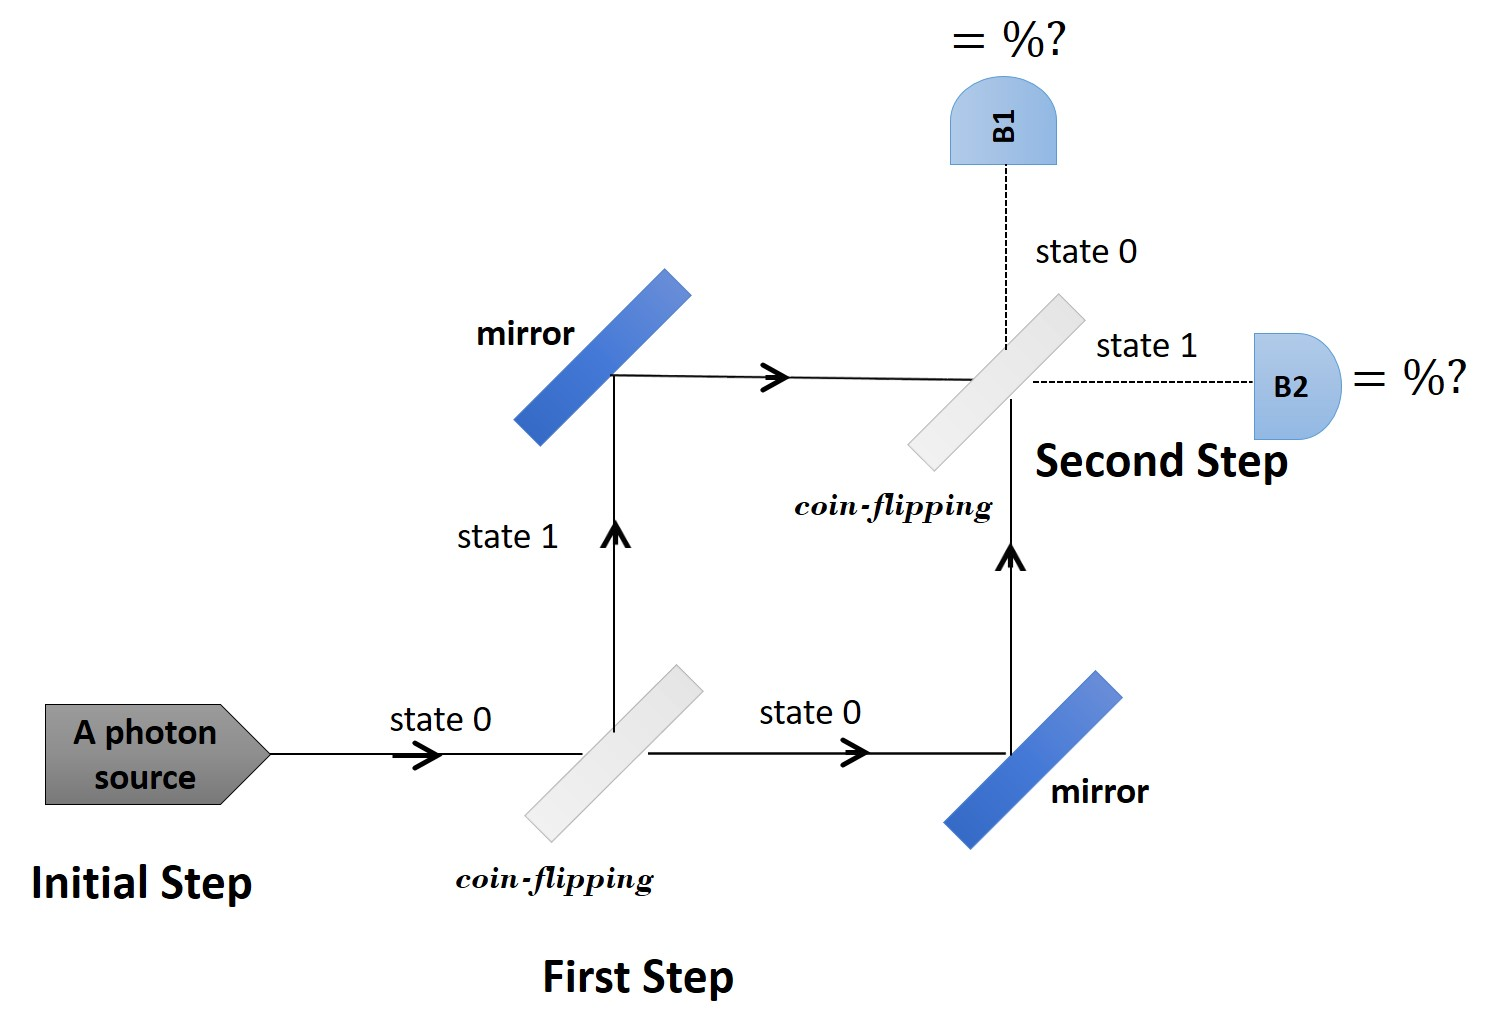
\includegraphics[width=320px]{qclass/images/photon6}
    \caption{Coin flipping}
    \label{fig:coin-flipping}
\end{figure}

Our prediction over the measures on B1 and B2 detectors of the Fig.~(\ref{fig:coin-flipping}) are $\%50$ on both.

However, the experiment results do not confirm our prediction.
We observe the photons only in the detector B1, and we never observe any photon in the detector B2.

How could this be possible?
We may conclude that the `classical' (Newtonian) mechanics fails to explain the behaviors of particles.